\documentclass[a4paper,11pt,openright]{book}
\usepackage[swapnames]{frontespizio}
%\usepackage[classica]{topfront}
%\usepackage[pdftex]{graphicx} %per poter inserire le figure
%\usepackage[a4paper,left=2cm,bottom=2cm,right=2cm,top=2cm]{geometry}
\usepackage{amssymb,amsmath,amsthm,amsfonts}
\usepackage{xspace}
\usepackage{indentfirst}
\usepackage{graphicx}
\usepackage{tabularx}
\usepackage[pdfa]{hyperref}
\usepackage[noabbrev,capitalize, italian]{cleveref}
\usepackage{subfigure}
\usepackage[small]{caption}
\usepackage{eucal}
\usepackage{eso-pic}
\usepackage{url}
\usepackage{booktabs}
\usepackage{afterpage}
\usepackage{parskip}
\usepackage{bookmark}
\usepackage{listings}
\usepackage{fancyhdr}
\usepackage{textcomp}
\usepackage{cite}
\usepackage{multirow}
\usepackage{adjustbox}
\usepackage[utf8]{inputenc}   %per riuscire a scrivere gli accenti
\usepackage[italian, english]{babel}   %per riuscire a scrivere gli accenti
\usepackage{setspace}


%%%%%%%%%%%
\newenvironment{abstract}%
{\cleardoublepage%
\thispagestyle{empty}%
\null \vfill
\begin{center}%
\Huge \bfseries \abstractname 
\end{center}}%
{\vfill\null}
%%%%%%%%%%%%%%%%%

%%%%%%%%%%%%%%%%%%%%%%%%%%%%%%%%%%%%%%%%%%%%%

% CONFIGURAZIONE LINK E RIFERIMENTI
\hypersetup{%
    pdfpagemode={UseOutlines},
    bookmarksopen,
    pdfstartview={FitH},
    colorlinks,
    linkcolor={black}, %COLORE DEI RIFERIMENTI AL TESTO
    citecolor={blue}, %COLORE DEI RIFERIMENTI ALLE CITAZIONI
    urlcolor={blue} %COLORI DEGLI URL
}

%%%%%%%%%%%%%%%%%%%%%%%%%%%%%%%%%%%%%%%%%%%%%%

\frenchspacing

%%%%%%%%%%%%%%%%%%%%%%%%%%%%%%%%%%%%%%%%%%%%%%

% INFORMAZIONI PDF - PERSONALIZZARE
\pdfinfo{%
  /Title    (Caratterizzazione spettroscopica del sistema di Didymos dopo l'impatto con la sonda DART)
  /Author   (Gabriele Bertinelli)
  /Subject  (Spettroscopia asteroide)
  /Keywords (spettroscopia, asteroide, Didymos, dart, rotazione)
}

%%%%%%%%%%%%%%%%%%%%%%%%%%%%%%%%%%%%%%%%%%%%%%





\begin{document}
\selectlanguage{italian}
\begin{frontespizio}

    \Universita{Padova}
    
    
    \Dipartimento{Fisica e Astronomia "Galileo Galilei"}
    
    
    \Corso[Laurea]{Astronomia}
    \Logo[3.0cm]{figure/UNIPD.png}
    
    
    {\Titoletto{Tesi di laurea triennale}}
    \Titolo{Caratterizzazione spettroscopica del sistema di\\ Didymos dopo l'impatto con la sonda DART}
    
    
    \Relatore{Prof.ssa Monica Lazzarin}
    \NRelatore{Relatrice}{}
    
    \Correlatore{Prof.ssa Fiorangela La Forgia}
    \NCorrelatore{Correlatrice}{}
    
    
    \Candidato{Gabriele Bertinelli}
    
    
   
    \Annoaccademico{2022-2023}
    
\end{frontespizio}



\frontmatter

\vspace*{\stretch{1}}
\begin{flushright}
\noindent
\textit{Alla mia famiglia}
\end{flushright}
\vspace*{\stretch{6}}
\cleardoublepage

\vspace*{\stretch{1}}
\begin{flushright}
\noindent
\textit{"Complete the motion if you stumble"}\\
\textit{RHCP}
\end{flushright}
\vspace*{\stretch{6}}
\cleardoublepage


\begin{abstract}    
Qui ci sarà il riassunto della tesi.\\
16 novembre 2022 è la data dell’inizio di una nuova era di missione spaziali: l’era delle missioni Artemis, che si ripromettono di riportare sulla Luna l’essere umano.

Alle 07:47, ora italiana, il razzo Space Launch System di NASA ha illuminato a giorno il pad 39-B al Kennedy Space Center, dando inizio alla missione Artemis I.
Scopo della missione è testare SLS nel suo complesso, razzo, capsula, sottosistemi, procedure ecc. 
Dopo 26 giorni di missione, l’11 dicembre, la capsula Orion rientrerà nell'Oceano Pacifico, al largo delle coste di San Diego.

Questa mattina, dopo qualche problema nei centri di controllo, il lancio è stato nominale: i booster migliorati, ereditati dalle missioni Shuttle, hanno performato bene; il core centrale di SLS (il cilindro arancione) idem; i 4 pannelli solari del Service Module, costruito dall’ESA (con grande contributo italiano) si sono aperti nel modo corretto e stanno generando la corrente elettrica necessaria.
Attorno alle 09:14 è iniziata la Trans Lunar Injection Maneuver, manovra per spostarsi dall'orbita terrestre a quella lunare, durata 18 minuti (un record per il motore RL10). Tutto è andato come previsto e Orion è in rotta verso la Luna.

I prossimi step sono la separazione dell'ICPS, il 2o stadio che ha permesso le ultime due manovre, correzioni dell’orbita e il rilascio di 13 cubesat, tra cui ArgoMoon: cubesat costruito da Argotec e ASI, azienda aerospaziale italiana, con l’obiettivo di monitorare da vicino tutte le operazioni che compirà la Orion attorno alla Luna.

Nei prossimi giorni seguiranno aggiornamenti sulla missione.
\end{abstract}



\tableofcontents

\listoftables

\listoffigures


\mainmatter

\chapter{Corpi minori del Sistema Solare}

\section{Proprietà generali}

Dal 1801, quando Giuseppe Piazzi scoprì il primo corpo minore Cerere, categorizzato poi come asteroide, per sottolineare le differenze apparenti rispetto alle comete, si sono scoperti e categorizzati più di 1 milione di asteroidi\footnote{\href{https://solarsystem.nasa.gov/asteroids-comets-and-meteors/asteroids/overview/}{https://solarsystem.nasa.gov/asteroids-comets-and-meteors/asteroids/overview/}} La maggior parte orbita tra Marte e Giove e forma quella che è chiamata Main Belt (2-3.3 AU).

Esistono numerosi gruppi di asteroidi, a diverse distanze dal Sole. Nella \cref{tab:asteroid-classification} sono riportati i principali gruppi e famiglie, con le loro classificazioni dinamiche.

In questo capitolo verranno descritte brevemente le principali caratteristiche. La loro definizione è spesso legata alla risonanza con Giove o Nettuno, mentre altri gruppi sono definiti dall'intersezione della loro orbita con quella di un pianeta (i.e. Near Earth Objects e Mars Crossers).

\subsection{Effetto Yarkovsky}
L’effetto Yarkovsky è una forza percepita da un corpo dovuta all’emissione anisotropa di fotoni termici, che trasportano momento. La sua influenza è più significativa per meteoroidi e piccoli asteroidi (da 10 cm a 10 km di diametro). %%ref 20 tesi balossi

L’effetto fu scoperto da Ivan Osipovich Yarkovsky, che notò come il riscaldamento diurno di un oggetto rotante nello spazio causasse una piccola forza sull’oggetto che avrebbe avuto effetti a lungo termine sulla sua orbita.

L’effetto è dovuto a due componenti:


\qquad \textit{Effetto diurno}: su un corpo rotante illuminato dal Sole, la superficie è più calda nel pomeriggio e nella prima parte della notte, rispetto alla mattina e a notte tarda. Il risultato è che viene radiato più calore dal lato notturno, rispetto a quello diurno, e, al netto, agisce una forza dovuta alla pressione di radiazione nella direzione opposta alla notte. Per oggetti rotanti in modo progrado, questa forza è nella direzione della loro orbita e il semiasse maggiore, nel lungo periodo, tende ad aumentare. Situazione opposta per gli oggetti che ruotano in modo retrogrado.


\qquad \textit{Effetto stagionale}: questa seconda tipologia tiene conto del fatto che nel corso di un anno uno dei due emisferi dell’asteroide risulta maggiormente esposto alla radiazione solare rispetto all’altro. Per oggetti rotanti, l’effetto stagionale aumenta con l’inclinazione assiale. Esso domina solo se l’effetto diurno è abbastanza piccolo.
%%ref 25 tesi balossi
L’effetto stagionale potrebbe avvenire per:

\begin{itemize}
    \item rotazione molto veloce
    \item piccole dimensioni dell’oggetto
    \item inclinazione assiale vicina a 90°
\end{itemize}

Anche questo effetto ha ripercussioni sul semiasse maggiore, e nell’ordine dei milioni di anni può portare un asteroide dalla Main Belt al Sistema Solare interno.

\begin{figure}
    \centering
    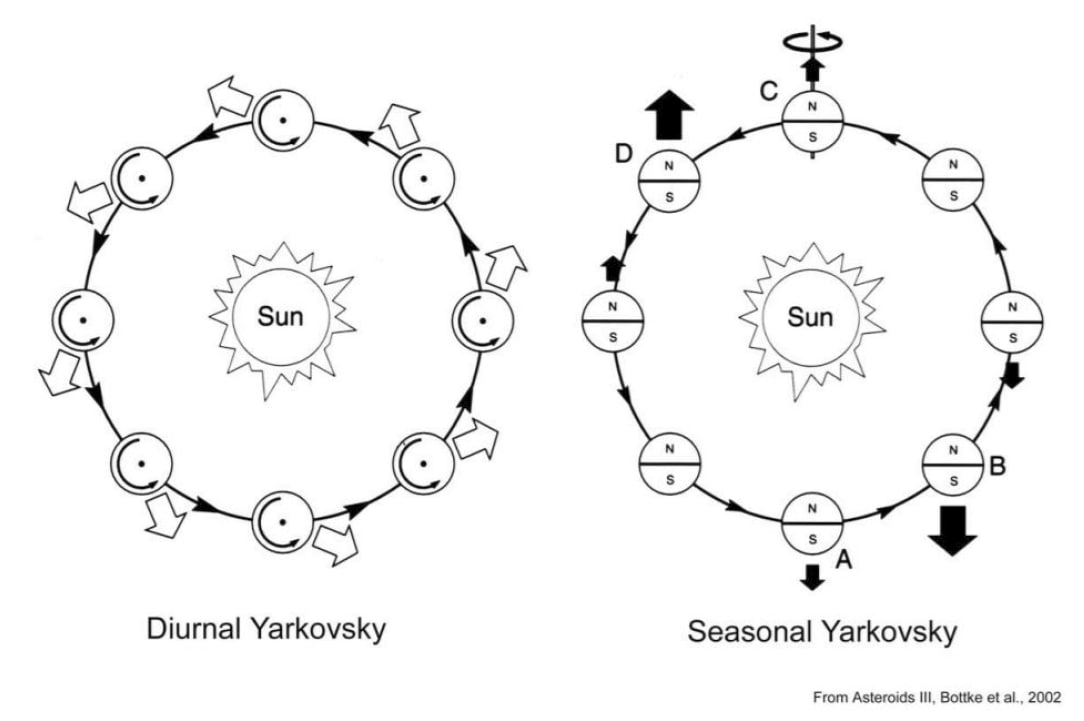
\includegraphics[scale=0.3]{figure/yark.jpg}
    \caption{Visualizzazione dell'effetto Yarkovsky diurno (a sinistra) e stagionale (a destra). (Credit: Bottkle et al., 2002)}
    \label{yark}
\end{figure}

\paragraph*{Effetto YORP}
L’effetto Yarkovsky-O'Keefe-Radzievskii-Paddack (YORP) è un variazione al secondo ordine dell’effetto Yarkovsky che causa l’aumentare o il diminuire della velocità di rotazione (o spin) di un piccolo corpo, come un asteroide.\\
Nel lungo termine, l'inclinazione e il tasso di rotazione dell'oggetto possono variare in modo casuale, in modo caotico o regolare, a seconda di molti fattori.

\section{Distribuzione e classificazione dinamica}
In questo capitolo verrà decritta la classificazione in gruppi e famiglie.
La classificazione è riassunta nella \cref{tab:asteroid-classification} .\\
I corpi minori sono divisi in gruppi e famiglie in base alle loro caratteristiche orbitali. 
Groups are relatively loose dynamical associations, whereas families are tighter e sono probabilmente il risultato di una distruzione catastrofica di un asteroide “genitore” (in inglese è tutto così bello “parent asteroid”).

Per la classificazione è utile conoscere le definizioni analitiche di afelio e perielio di un'orbita:
\begin{equation}
    \begin{cases}
        Q=a(1+e) &\text{afelio}\\
        q=a(1-e) &\text{perielio}
    \end{cases}
\end{equation}

dove \textit{a} e \textit{e} sono rispettivamente il semiasse maggiore e l'eccentricità dell'orbita.

\paragraph*{Near Earth Objects}
I Near Earth Objects (NEOs) rappresentano un gruppo eterogeneo di asteroidi (NEAs) e nuclei cometari estinti (NECs) che hanno orbite con un perielio minore di quello di Marte: $q<1.3$ AU. Si ritiene che i NEOs siano la principale fonte di meteoriti che arrivano sulla Terra.\\
In base alla relazione tra la loro orbita e quella della Terra sono catalogati in diversi sotto-gruppi: \textit{Atens} e \textit{Apollo} sono Earth Crossers (i.e. intersecano l’orbita della Terra), mentre gli \textit{Amors} si avvicinano alla Terra ma non intersecano mai la sua orbita. Gli Atens hanno un semiasse maggiore più piccolo di quello della Terra ($a<1$ AU) mentre gli Apollo hanno $a>1$ AU.


\begin{table}
    
    \begin{center}
    \resizebox{\linewidth}{!}{%
    
    \begin{tabular}{cccccc}
      \toprule
      \toprule
      \bf{Popolazione} & \bf{Famiglia/Gruppo} & \bf{a}     & \bf{q}     & \bf{Q}     & \bf{Commento} \\
      \midrule
      NEAs        &                 &       &       &       &           \\
                  & Atens           & $<1$  &              & $\geq 0.983$ & Earth Crossers     \\
                  & Apollos         & $>1$  & $\leq 1.017$ &              & Earth Crossers \\
                  & Amors           & $>1$  & $(1.017,1.3)$ &             &  \\
      \midrule
      Mars Crossers &               &       & $[1.3,1.67]$ &             &  \\
      \midrule
      \midrule
      \bf{Popolazione} & \bf{Famiglia/Gruppo} & \bf{a}     & \bf{e}     & \bf{i}     & \bf{Risonanze} \\
      \midrule
      Main Belt Asteroids &       &       &       &       &  \\
            & Hungarians & $[1.78,2.06]$ & $<0.18$ & $[16,34]$ & $[5:1, 4:1]$ \\
            & Inner MB & $[2.06,2.50]$ &       & $[18,32]$ & $[4:1,3:1]$ \\
            & Middle MB & $[2.50,2.82]$ &       &       & $[3:1,5:2]$ \\
            & Outer MB & $[2.82,3.28]$ &       &       & $[5:2,2:1]$ \\
            & Cybeles & $[3.28,3.70]$ & $<0.3$ & $<25$ & $[2:1,5:3]$ \\
            & Hildas & $\sim 3.97$ & $>0.07$ & $<20$ & $3:2$ \\
      \midrule
      Jupiter Trojans &       & $\sim 5.20$ &       &       & $1:1$ \\
      \midrule
      Centaurs &       & $[5.4,30]$ &       &       &  \\
      \midrule
      Neptune Trojans &       & $\sim 30$ &       &       & 1:1 Nep \\
      \midrule
      TNOs (o KBOs) &       & $>32$ &       &       & $[4:5, 2:3]$ \\
            &       &       &       &       & $[3:5, 1:2]$ \\
      \bottomrule
      \bottomrule
    \end{tabular}}%
    \end{center}
    \caption[Lista e definizioni delle principali popolazioni di asteroidi]{Lista e definizioni dei principali gruppi e famiglie di asteroidi. Il semiasse maggiore $a$, il perielio $q$ e l'afelio $Q$ sono espressi in AU; l'inclinazione $i$ in gradi. $e$ è l'eccentricità. Le risonanze, dove non è indicato, si riferiscono all'orbita di Giove.}
    \label{tab:asteroid-classification}
\end{table}%
  

\paragraph*{Mars Crossers}
Come fa intendere il nome, i \textit{Mars Crossers} sono oggetti che intersecano l’orbita di Marte.\\
È stato mostrato che la popolazione dei Mars Crossers, che è circa 4 volte più grande di quella dei NEOs, è rifornita da risonanze diffusive nella Main Belt (Migliorini et al. 1998; Morbidelli \& Nesvorny 1999; Michel et al. 2000; Bottke et al. 2002), dalla regione chiamata “intermediate-source Mars-crossing region” o IMC.

\paragraph*{Main Belt Asteroids}
Si tratta di asteroidi situati tra le orbite di Marte e Giove. La maggior concentrazione si trova tra 2.0 e 3.3 AU.\\
A causa delle risonanze orbitali dovute all’influenza gravitazionale di Giove, si vengono a creare molti gruppi, sotto-gruppi e famiglie. Di seguito sono riportati i più popolosi.

\qquad \textit{Hungaria}: prendono il nome da (434) Hungaria. Hanno un semiasse maggiore tra 1.78 e 2.06 AU, un’eccentricità minore di 0.18 e un’inclinazione tra 16° e 34°. 

\qquad \textit{Inner Main Belt}: hanno un semiasse maggiore tra 2.06 e 2.50 AU, limiti definiti dalle risonanze di moto medio 4:1 e 3:1.

\qquad \textit{Middle Main Belt}: hanno un semiasse maggiore tra 2.50 e 2.82 AU. I limiti sono definiti dalle risonanze di moto medio 3:1 e 5:2.

\qquad \textit{Outer Main Belt}: hanno un semiasse maggiore tra 2.82 e 3.28 AU. All’interno del gruppo troviamo le famiglie \textit{Koronis}, \textit{Eos} e \textit{Themis}.

\qquad \textit{Cybele}: hanno un semiasse maggiore tra 3.28 e 3.70 AU. Prendono il nome da (65) Cybele.

\qquad \textit{Hilda}: hanno un semiasse maggiore medio tra 3.70 e 4.20 AU. Prendono il nome da (153) Hilda.

\paragraph*{Jupiter Family Comets}
Le comete sono divise in due gruppi: comete a lungo periodo e comete a corto periodo.\\
Le comete a corto periodo hanno un periodo orbitale $< 20$ anni a basse inclinazioni. Hanno anche $2<T_J<3$, con $T_J$ Invariante di Tisserand, espressa da

\begin{equation}
    T_J=\frac{a_J}{a}+2\cos(i)\biggl[\frac{a}{a_J}(1-e)\biggr]^{1/2}
\end{equation}

dove $a$ e $a_J$ sono i semiassi maggiori dell'oggetto e di Giove rispettivamente ed $e$ è l'eccentricità dell'oggetto.\\
Visto che la loro orbita è controllata da Giove sono chiamate Jupiter Family Comets (JFCs). Si pensa che le comete a corto periodo provengano dalla Kuiper Belt, una grande riserva di piccoli corpi ghiacciati che si trova oltre Nettuno. A causa di collisioni e/o perturbazioni gravitazionali alcuni oggetti della Kuiper Belt riescono a fuggire dalla stessa e dirigersi verso il Sistema Solare interno. La successiva interazione con Giove può far sì che questi oggetti assumano parametri orbitali simili a quelli degli asteroidi.

\paragraph*{Centaurs}
I Centaurs sono oggetti che orbitano tra Giove e Nettuno ($5.4<a<30$ AU), ma non hanno ancora una definizione dinamica univoca.\\
Studi dinamici delle loro orbite indicano che i centaurs sono probabilmente degli oggetti con caratteristiche orbitali intermedie tra quelli della Kuiper Belt e le JFCs.\\
Sono probabilmente più simili a comete che ad asteroidi, e uno di questi, Chiron, è stato osservato avere attività cometaria.

\paragraph*{Trans Neptunian Objects}
Sono oggetti con $a\geq 30$ AU e sono divisi nei seguenti gruppi:

\qquad \textit{Kuiper Belt Objects}: si trovano tra 41 e 47 AU. A sua volta si divide nei sotto-gruppi dei \textit{Plutinos}, in risonanza 3:2 con Nettuno come Plutone e dei \textit{Cubewanos}, conosciuti come i classici KBOs.

\qquad \textit{Scattered-Disk Objects (SDOs)}: hanno orbite molto grandi e molto ellittiche, probabilmente dovute a un’interazione con Nettuno.

\qquad \textit{Oort Cloud Objects (OCOs)}: la Oort Cloud è una shell sferica di oggetti ghiacciati, di cui non si ha evidenza diretta perché troppo lontana e scura ma ipotizzata come luogo di origine delle comete a lungo/lunghissimo periodo. Si trova tra circa 50000 e 100000 AU.

\section{Potentially Hazardous Asteroids (PHA)}
Tra i NEO esiste una categoria di oggetti che riveste un ruolo importante: sono gli asteroidi potenzialmente pericolosi, Potentially Hazardous Asteroids (PHA). Rientrano in questa categoria tutti gli oggetti la cui minima distanza all'intersezione dell'orbita terrestre (Minimum Orbit Intersection Distance - MOID) è inferiore a 0.05 AU e la cui magnitudine assoluta H è minore di 22. Sono, quindi, quegli asteroidi che se impattassero con la Terra provocherebbero danni su larga scala, anche globale. Ad oggi si conoscono più di 2500 PHA, la maggior parte dei quali sono della famiglia Apollo, e ogni giorni vengo aggiunti o rimossi oggetti sulla base di nuovi risultati sulla base dei parametri orbitali.\\
La determinazione dell'orbita avviene sulla base delle osservazioni disponibili ed è definita da sei parametri orbitali, influenzati da diversi fattori. Quindi non si può determinare immediatamente con sufficiente accuratezza l'orbita ma servono osservazioni costanti nel tempo.\\
Al momento della scoperta di un PHA si determina l'orbita per i successivi 100 anni. Si possono determinare in tal modo i passaggi ravvicinati (fly-by) che l'asteroide avrà con la Terra e, conoscendo la regione di incertezza, la probabilità di collisione con la stessa.
I PHA con una probabilità non nulla di impatto con la Terra nei futuri 100 anni vengono catalogati nella Sentry Risk Table\footnote{\href {https://cneos.jpl.nasa.gov/sentry/}{https://cneos.jpl.nasa.gov/sentry/} }, un sistema informatico gestito dal CNEOS (Center for Near-Earth Object Studies).\\
Oltre alla probabilità di collisione e alcune caratteristiche dell’oggetto (magnitudine assoluta, diametro) nella \cref{tab:asteroid-classification} vengono riportati i valori dell’asteroide sulla Scala Torino e Scala Palermo. Queste sono due classificazioni che permettono di quantificare il pericolo associato ad ogni asteroide: la Scala Torino è stata pensata per la comunicazione al pubblico, la Scala Palermo è più tecnica e viene usata direttamente dagli astronomi.
%%direi che ha poco senso mettere due paragrafi sulla scala milano e torino, ma non costa nulla

\chapter{Spettroscopia}

\section{Introduzione}
Lo studio della mineralogia superficiale di singoli asteroidi o di gruppi di asteroidi può fornire i dati per migliorare la nostra comprensione della loro origine ed evoluzione. La superficie degli asteroidi può essere studiata dall'interpretazione delle proprietà osservabili per determinare la presenza, l'abbondanza e la composizione mineralogica.\\
La spettroscopia di riflettanza nel visibile (VIS) e nell'infrarosso (IR) viene ampiamente usata per determinare la composizione degli asteroidi poiché può caratterizzare la composizione superficiale della maggior parte dei tipi di asteroidi. Le caratteristiche diagnostiche negli spettri, che derivano da transizioni elettroniche e vibrazionali all'interno dei minerali e delle molecole, sono riscontrabili nell'intervallo di frequenza $0.35-2.50\,\mu m$.\\
I minerali più importanti presenti negli spettri degli asteroidi sono: olivine, pirosseni, metalli Ferro-Nichel, feldspati e fillosilicati idrati e composti organici.\\
La maggior parte degli asteroidi è composta da un mix di questi minerali. Poiché i parametri spettrali dei diversi assorbimenti (i.e. la posizione delle bande e il rapporto tra esse) sono legati a una specifica composizione del singolo minerale, l'analisi spettrale della superficie degli asteroidi è in grado, nella maggior parte dei casi, di rilevare le firme mineralogiche caratteristiche di una particolare specie.\\
La possibilità di rilevare una feature dipende dall'abbondanza della particolare specie, in modo che la forza della feature possa essere rilevata sopra il rumore dello spettro.\\
In spettri di alta qualità può essere anche determinata la composizione e le relative abbondanze di un mix di minerali.\\
Per questi motivi l'analisi degli spettri può fornire una varietà di dati sulla composizione della superficie degli asteroidi.

\section{Spettro degli asteroidi}
Il flusso incidente che arriva sulla superficie di un asteroide è diviso in due contributi: la parte riflessa e la parte assorbita, il cui rapporto dipende dall'albedo. La parte assorbita riscalda la superficie del corpo. Questo emette, di conseguenza, radiazione di corpo nero determinata dalla temperatura raggiunta. Quindi la Terra riceve sia il flusso "solare" riflesso dall'oggetto che la radiazione di corpo nero.\\
Negli spettri degli asteroidi la radiazione solare riflessa domina nel range che va dall'ultravioletto (UV) al vicino infrarosso (NIR): $0.35-2.50\,\mu m$; mentre a lunghezze maggiori ($2.5-5.0\,\mu m$) il contributo della radiazione di corpo nero dell'asteroide diventa rilevabile.

\section{Tipi tassonomici}
La tassonomia è la classificazione degli oggetti in categorie definite da alcuni parametri caratterizzanti. Sin dagli anni '70 diversi autori hanno creato diverse classi tassonomiche basandosi su proprietà osservabili.\\
La classificazione tassonomica più utilizzata è quella di Tholen (1984), basata su più di 400 spettri ricavati dalla Eight-Color Asteroid Survey (ECAS), nel range spettrale $0.3-1.1\,\mu m$. Dagli spettri ECAS si possono distinguere undici classi spettrali (A, B, C, D, F, G, Q, R, S, T e V).\\
Barucci et al., nel 1987, usarono sette colori spettrofotometrici e gli albedo ricavati dalle survey IRAS per definire nove classi spettrali e per ognuna delle sottoclassi identificate dallo studio dettagliato degli spettri.\\
Infine, Bus e Binzel (Bus \& Binzel (2002b), Bus \& Binzel (2002a)) hanno derivato la loro classificazione tassonomica da dati spettrofotometrici recenti.

\subsection{Tassonomia di Tholen}
Ognuna delle tassonomie menzionate sopra separa gli asteroidi in diverse classi secondo riflettività e albedo visuali (nel visibile) simili. Sebbene non viene usato nessun criterio mineralogico nel definire le classi, la tassonomia può essere usata per derivare la caratterizzazione mineralogica di ogni asteroide nelle varie classi.\\
Di seguito descriveremo brevemente le principali caratteristiche di ogni classe della tassonomia di Tholen e la loro relazione con le meteoriti.

\paragraph*{Classe A}
Gli asteroidi di tipo A mostrano una forte decrescita nella riflettanza attorno a $0.7\,\mu m$, relativa a composti metallici, e un forte banda di assorbimento centrata attorno a $1\,\mu m$ e nessun assorbimento rilevante a $2\,\mu m$ (caratteristica dei pirosseni).\\
Sono asteroidi molto rari, situati principale nella Main Belt interna. Si ritiene che questi oggetti siano frammenti del mantello differenziato di corpi progenitori di dimensioni maggiori.\\
Le analoghe meteoriti sono le acondrite a olivina e/o pallasite.

\begin{figure}
\centering
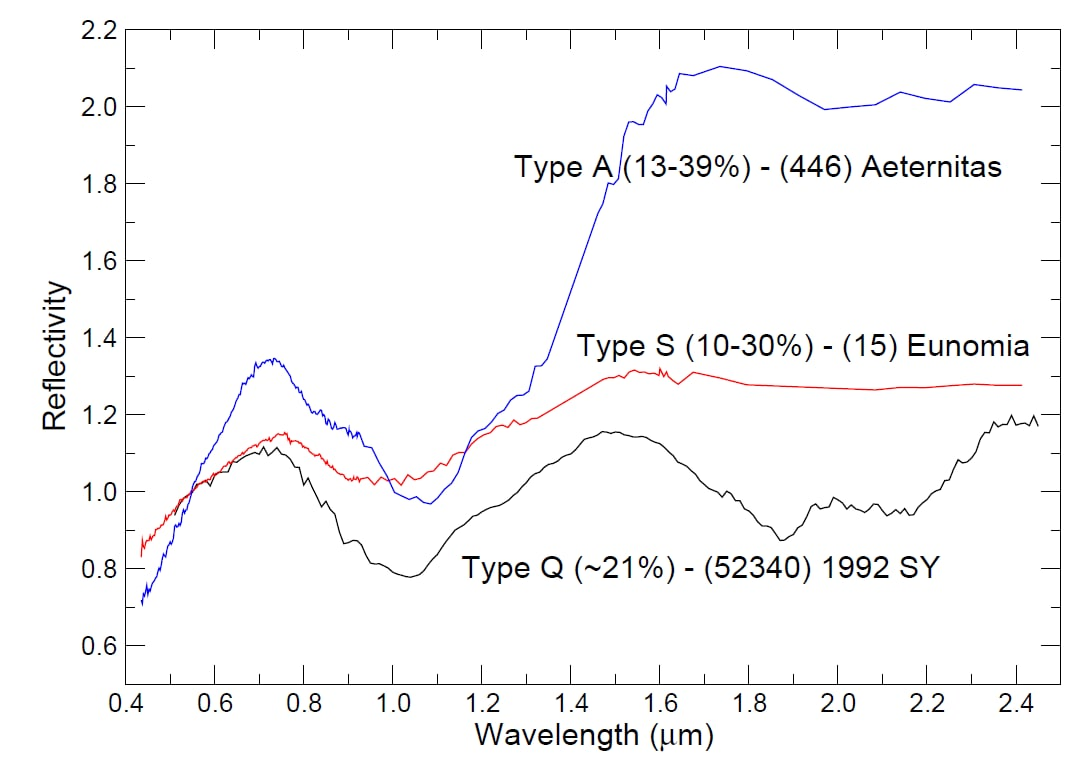
\includegraphics[scale=0.3]{figure/spettro_qsa.jpg}
\caption{Esempio di spettri di tipo Q, S e A. Gli spettri sono normalizzati a $0.55\,\mu m$. Tra parentesi è riportato il range di albedo in percentuale. (Magrin, 2006)}
\label{spettro_qsa}
\end{figure}

\paragraph*{Classe S}
Rappresenta la seconda classe più numerosa ed è caratterizzata da spettri con una pendenza ripida attorno a $0.7\,\mu m$ e assorbimenti moderati attorno a $1$ e $2\,\mu m$. La loro albedo varia tra $0.1$ e $0.3$. Lo spettro tipico degli asteroidi di tipo S indica la presenza di un mix di olivine, pirosseni e metalli Fe-Ni; in particolare di silicati: ciò li rende i corpi progenitori più probabili per le meteoriti rocciose.\\
A causa della classificazione di Tholen sono stati introdotti diversi sottogruppi definiti in base alle diverse composizioni e storie evolutive degli asteroidi.\\
Gli asteroidi di tipo S sono situati principalmente nella Main Belt interna e diventano più rari spostandosi verso l'esterno.

\paragraph*{Classe Q}
È una classe di oggetti molto scarna, i pochi corpi di questo tipo sono NEO ma nessuno appartiene alla Main Belt. Un ottimo rappresentante della classe è il NEO (1862) Apollo. Lo spettro è fortemente arrossato attorno a $0.7\,\mu m$ e ha due forti assorbimenti a $1$ e $2\,\mu m$, caratteristiche proprie di un mix di olivine e pirosseni.\\
Questi spettri sono simili a quelli delle condriti ordinarie (CO), che rappresentano circa l'80\% delle meteoriti trovate sulla superficie terrestre. Ciò indicherebbe che gli asteroidi di tipo Q siano i progenitori di queste meteoriti e quindi dovrebbero essere molto numerosi, in contrasto con le osservazioni.

\paragraph*{Classe R}
Questa classe fu inizialmente proposta unicamente per (349) Dembowska. Il suo spettro mostra forti assorbimenti a $1$ e $2\,\mu m$, simili a quelli di Vesta. Dembowska, a differenza di Vesta, presenta caratteristiche allargate verso lunghezze d'onda maggiori, mentre l'assorbimento a $2\,\mu m$ è più stretto e centrato su lunghezze d'onda minori.\\
Le caratteristiche spettrali indicano la presenza di olivine e pirosseni (circa in eguali quantità) e pochi o alcun metalli. 

\begin{figure}
    \centering
    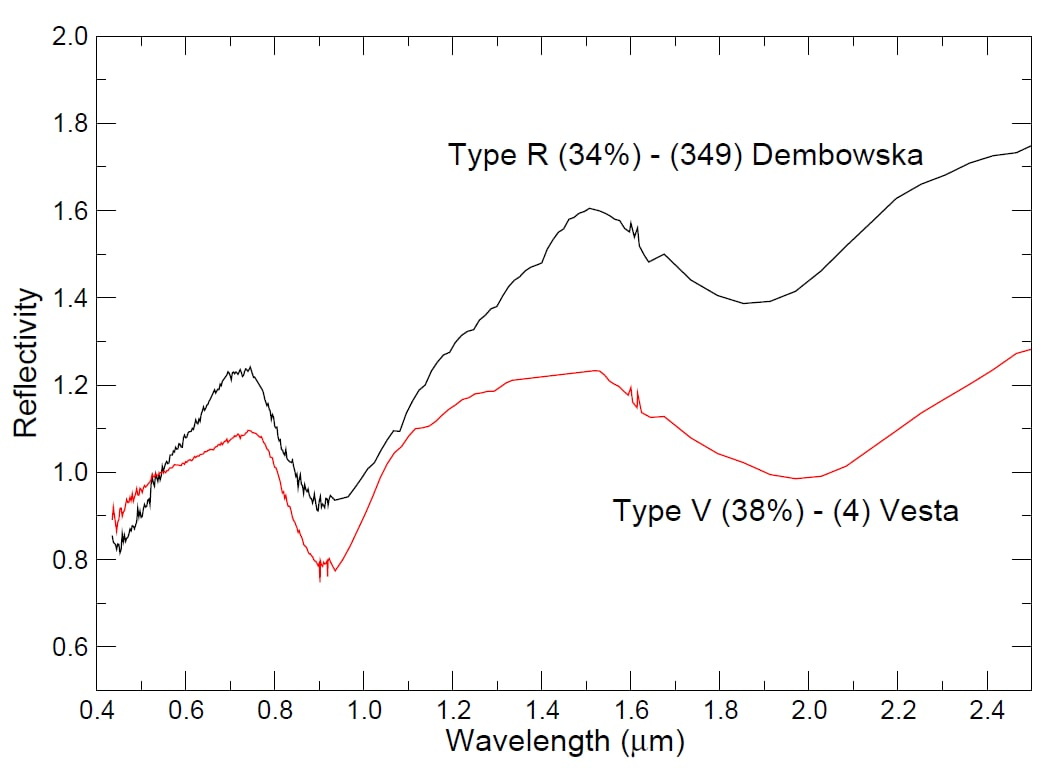
\includegraphics[scale=0.3]{figure/spettro_rv.jpg}
    \caption{Esempio di spettri di tipo V e R. Gli spettri sono normalizzati a $0.55\,\mu m$. Tra parentesi è riportato il range di albedo in percentuale. (Magrin, 2006)}
    \label{spettro_rv}
\end{figure}

\paragraph*{Classe V}
Questa classe fu proposta per (4) Vesta. Il suo spettro è caratterizzato da forti assorbimenti centrati vicino a $1$ e $2\,\mu m$, dovuti ai pirosseni.\\
All'incirca il 6\% degli asteroidi della Main Belt rientra all'interno di questo gruppo. La maggior parte degli asteroidi di tipo V, noti come vestoidi, orbitano nelle vicinanze di Vesta, il che suggerisce che siano dei suoi frammenti generatisi in seguito a impatti con altri corpi. Alcuni NEA sono risultati essere vestoidi: ciò dimostra l'efficacia dei meccanismi di trasporto degli asteroidi dalla Main Belt alle regioni del Sistema Solare interno.

\paragraph*{Classe C}
In letteratura ci si riferisce al gruppo C come un grande gruppo di oggetti scuri e primitivi. Contiene infatti circa il 75\% degli asteroidi noti. Questi oggetti dominano nelle regioni esterne della Main Belt, dove compongono l'80\% di tutta la popolazione, ma diventano più rari spostandosi verso l'interno.\\
Gli asteroidi di tipo C non presentano alcuna caratteristica attorno a $0.4\,\mu m$ ma hanno diverse intensità di assorbimento nell'UV. All'interno di questa classe sono state introdotte le sottoclassi C, B, F, G e P.\\
La classe P non ha assorbimenti nell'UV, la classe F ne ha uno debole, B e C leggermente più intenso e la classe G ha l'assorbimento UV più intenso di tutto il gruppo C. La classe B ha uno spettro da piatto e leggermente blu mentre la classe C da piatto a leggermente rosso. Bell et al. (1989) ha proposto un modello per interpretare le diversità nel gruppo C: le classi B, F e G sarebbero il risultato di un'alterazione metamorfica di un progenitore di classe C. La classe P, che si trova principalmente nella parte esterna della Main Belt, si pensa sia costituita da materiale primitivo contenente una gran quantità di materiale organico, e potrebbe essere una classe di transizione tra C e gli oggetti molto primitivi della classe D.\\
Circa due terzi degli oggetti del gruppo C appaiono idratati, dall'analisi dello spettro attorno a $3\,\mu m$ e nella regione del visibile, probabilmente perché sono stati scaldati al punto che acqua liquida è entrata in contatto con il materiale circostante.

\paragraph*{Classe D}
Gli spettri degli asteroidi di classe D sono generalmente senza caratteristiche particolari, con spettri tendenti leggermente verso il rosso attorno a $0.55\,\mu m$ e spettri molto rossi dopo $0.55\,\mu m$. Hanno, inoltre, albedo molto bassi ($\leq 0.05$).\\
Sono situati nella Main Belt esterna e tra i Troiani di Giove, di cui costituiscono il 60\% della popolazione totale. È stato ipotizzato che questi asteroidi siano composti da una complessa miscela di materiale organico e di regolite\footnote{La regolite è uno strato di frammenti rocciosi incoerenti che forma il terreno superficiale dei vari oggetti nel Sistema Solare.} e che provengano dalla Kuiper Belt.

\begin{figure}
    \centering
    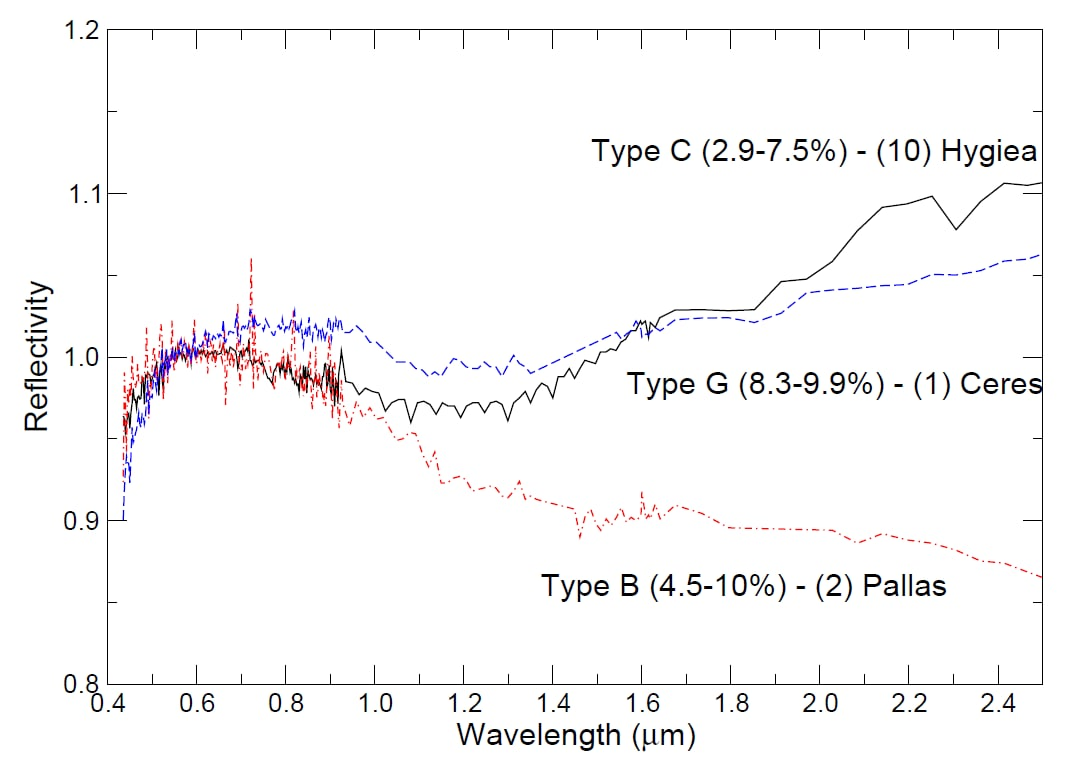
\includegraphics[scale=0.3]{figure/spettro_bgc.jpg}
    \caption{Esempio di spettri di tipo B, G e C. Gli spettri sono normalizzati a $0.55\,\mu m$. La scala verticale è ampliata per rendere apprezzabili le differenze tra le classi. Tra parentesi è riportato il range di albedo in percentuale. (Magrin, 2006)}
    \label{spettro_bgc}
\end{figure}

\begin{figure}
    \centering
    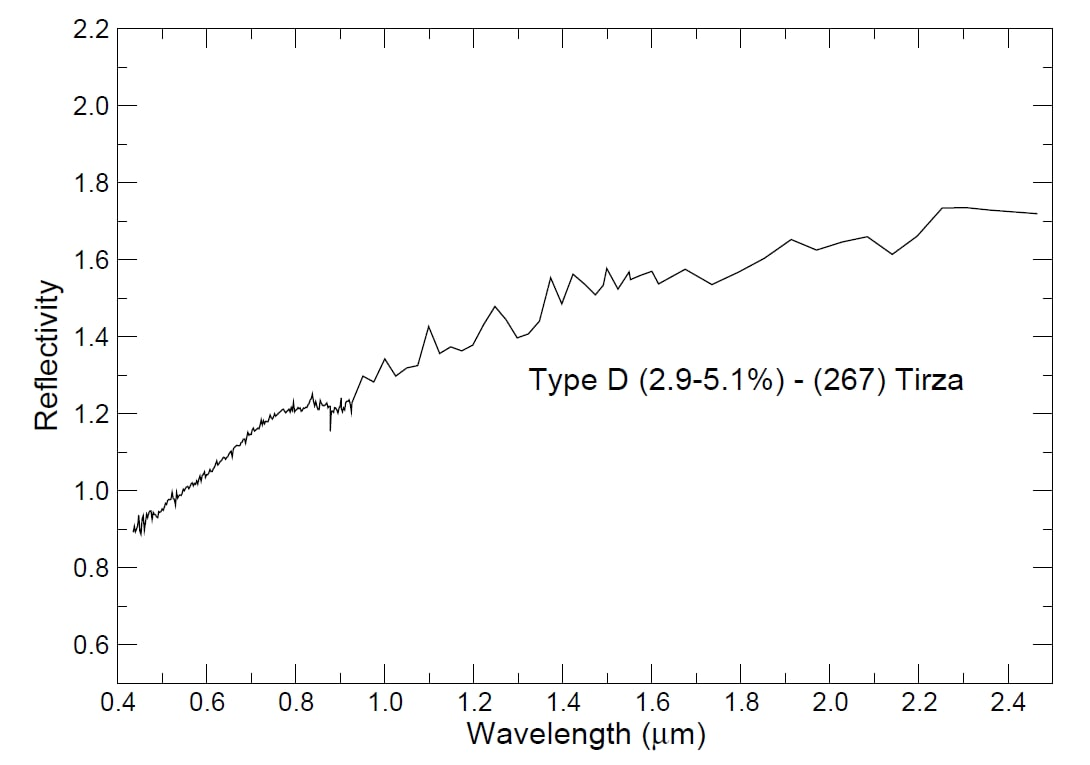
\includegraphics[scale=0.3]{figure/spettro_d.jpg}
    \caption{Esempio di spettro di tipo D. Lo spettro è normalizzato a $0.55\,\mu m$. Tra parentesi è riportato il range di albedo in percentuale. (Magrin, 2006)}
    \label{spettro_d}
\end{figure}

\paragraph*{Classe E}
GLi asteroidi di classe E hanno uno spettro senza caratteristiche, molto simile a quello della classe M. Si differenziano da questi ultimi per via della loro elevata albedo, superiore a $0.3$. La composizione superficiale dovrebbe essere costituita da silicati poveri di ferro, come enstatite e feldspato.\\
Il gruppo degli Hungaria contiene la metà degli asteroidi di classe E noti. Si crede che alcuni NEO di questo gruppo siano i corpi progenitori delle aubriti, una sottoclasse delle meteoriti acondriti.

\begin{figure}[h]
    \centering
    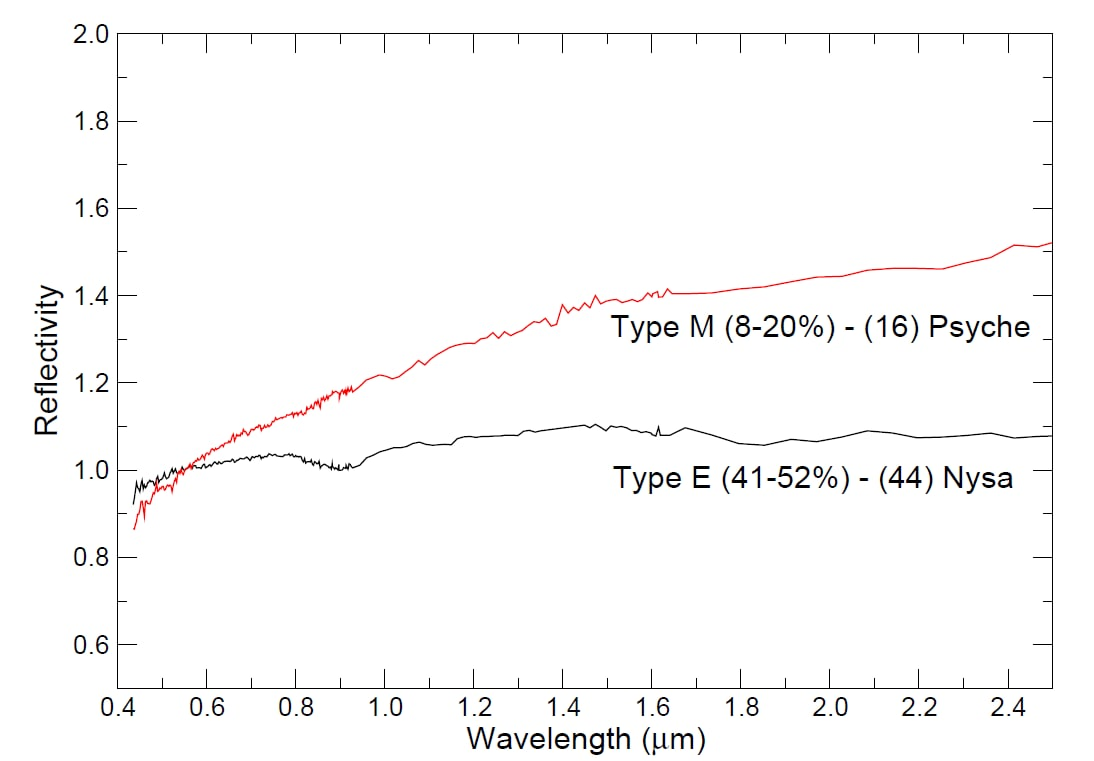
\includegraphics[scale=0.3]{figure/spettro_em.jpg}
    \caption{Esempio di spettri di tipo E e M. Gli spettri sono normalizzati a $0.55\,\mu m$. Tra parentesi è riportato il range di albedo in percentuale. (Magrin, 2006)}
    \label{spettro_em}
\end{figure}

\paragraph*{Classe M}
Si tratta del terzo gruppo più numeroso. Gli spettri sono caratterizzati da un leggero arrossamento e senza particolari caratteristiche. Gli asteroidi di questa classe hanno albedo comprese tra $0.1$ e $0.2$. I dati suggeriscono che la composizione è principalmente ferro e nichel, suggerendo che questi oggetti siano i nuclei metallici differenziati di oggetti più grandi andati distrutti. Si ritengono essere quindi i progenitori delle meteoriti metalliche.

\paragraph*{Classe T}
Gli asteroidi di classe T sono molto rari e hanno albedo molto basse ($\leq 0.1$) con spettri leggermente rossi vero $0.85\,\mu m$. Si ritiene che siano composti da materiale carbonaceo fortemente
alterato (o termicamente o dall'azione dell'acqua).

\begin{figure}
    \centering
    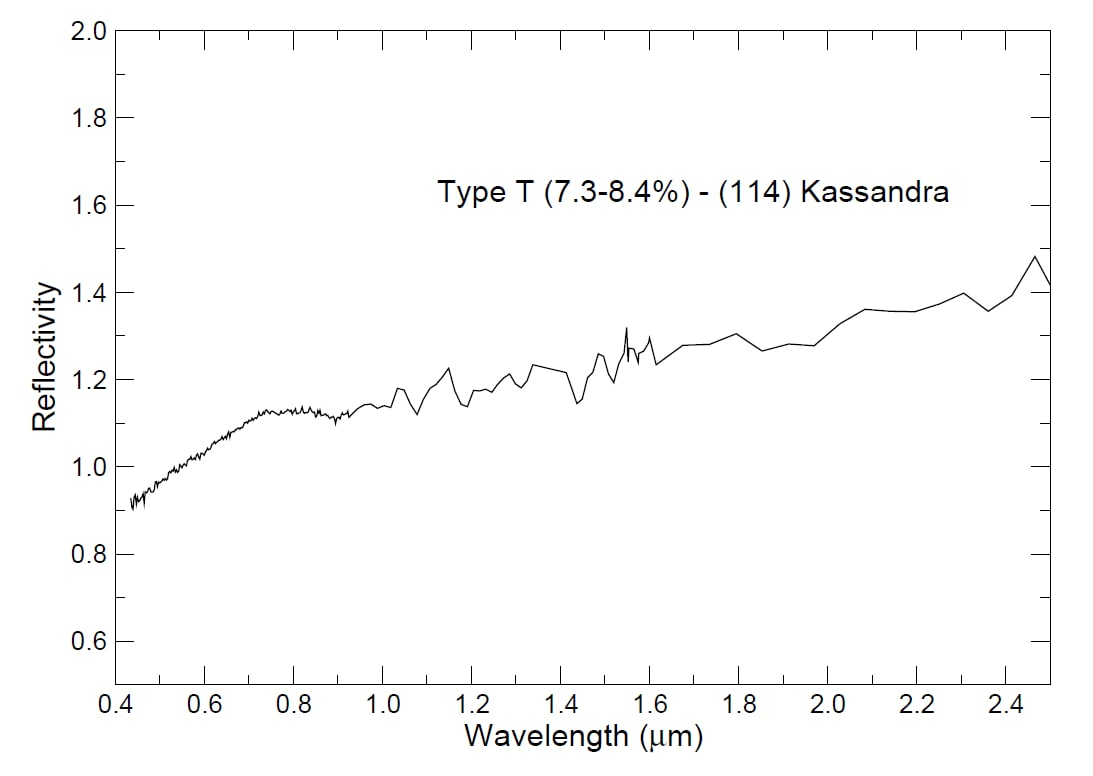
\includegraphics[scale=0.3]{figure/spettro_t.jpg}
    \caption{Esempio di spettro di tipo T. Lo spettro è normalizzato a $0.55\,\mu m$. Tra parentesi è riportato il range di albedo in percentuale. (Magrin, 2006)}
    \label{spettro_t}
\end{figure}

\subsection{Tassonomia di Bus}
I dati della SMASSII\footnote{\href{http://smass.mit.edu/smass.html}{http://smass.mit.edu/smass.html}} (Small Main-Belt Asteroid Spectroscopic Survey) hanno fornito delle nuove base oer una tassonomia. Bus \& Binzel (2002b) and Bus \& Binzel (2002a) hanno costruito il loro sistema di classificazione basandosi sulle tassonomie pre-esistenti. In particolare hanno definito tre gruppi principali: S-, C- e X-complex, corrispondenti alle definizioni classiche dei tipi S, C e X. Di conseguenza sono state definite 26 classi sulla base della presenza o assenza di alcune caratteristiche spettrali. Di queste 26 classi, 12 hanno una designazione a una lettera: A, B, C, D, K, O, Q, R, S, T, V e X. Una nuova classe, la L, è stata introdotta per descrivere gli oggetti con una pendenza molto ripida nell'UV, vicino a $0.75\,\mu m$, ma con uno spettro piatto oltre i $0.75\,\mu m$. Asteroidi con caratteristiche intermedie sono associati a classi multi-lettera: Cb, Cg, Cgh, Ch, Ld, Sa, Sk, Sl, Sq, Sr, Xc, Xe, e Xk. I membri delle classi Cgh- e Ch- hanno spettri contenenti un assorbimento a $0.7\,\mu m$ legato all'idratazione.\\
Un nuovo asteroide può quindi venire facilmente classificato all’interno di una di queste classi solamente sulla base delle sue caratteristiche spettrali. Di seguito un riassunto delle chiavi tassonomiche della classificazione di Bus-DeMeo.

\begin{figure}[h]
    \centering
    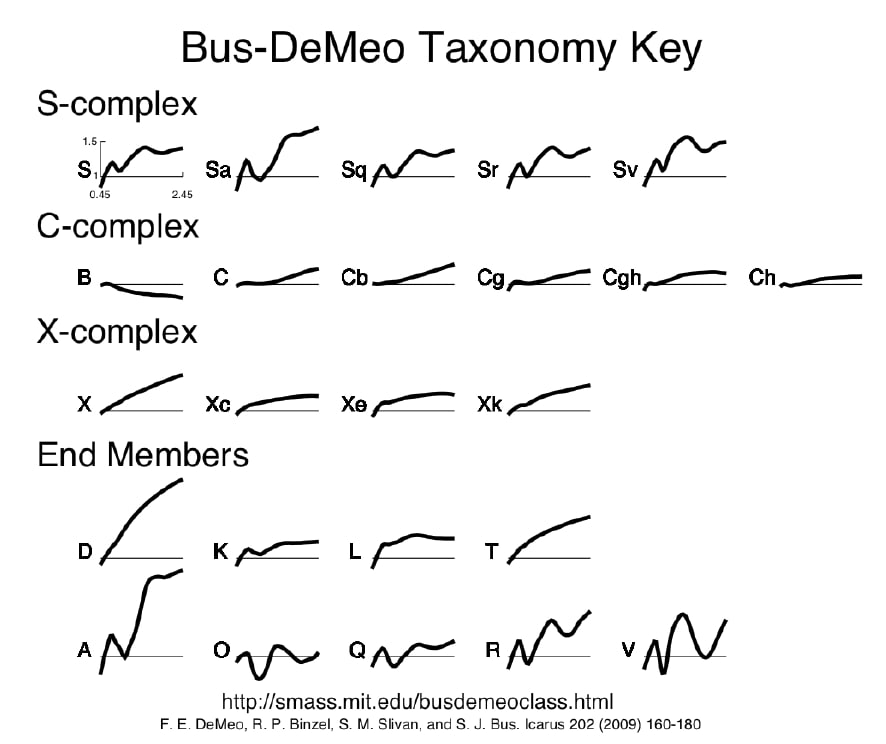
\includegraphics[scale=0.44]{figure/spettro_bus.jpg}
    \caption{Spettri dei tipi tassonomici introdotti da Bus e Binzel. (DeMeo et al., 2009)}
    \label{spettro_bus}
\end{figure}
\section{Space Weathering (foorse)}

























\end{document}